\section{Linguaggi ed espressioni regolari}
I \emph{linguaggi regolari} sono la famiglia più semplice di linguaggi formali, questo perchè possono essere definiti in diversi modi:
\begin{itemize}
	\item Algebricamente.
	\item Attraverso grammatiche generative.
	\item Attraverso algoritmi di riconoscimento (\emph{automi})
\end{itemize}
Le \emph{espressioni regolari} (\emph{regexp}) sono stringhe \emph{r} definite attraverso i caaratteri di un alfabeto $ \Sigma $ e mediante l'utilizzo dei metasimboli $ \varnothing, \cup, \cdot, \ast $ attraverso l'applicazione e la combinazione delle seguenti regole
\begin{itemize}
	\item $ r= \varnothing $
	\item $ r = a, a\in \Sigma $
	\item $ r = (s \cup t) $
	\item $ r = (s\cdot t) \ o \ r = (st) $
	\item $ r = (s)^\ast $
\end{itemize}
Oltre a questi simboli talvolta, per semplificare la notazione, si utilizzano anche i simboli $ \varepsilon = \varnothing^\ast$ e $ r^+ = e\cdot e^\ast $.\\
Il risultato di un'espressione regolare \emph{e} è un linguaggio $ L_e $ costruito sull'alfabeto $ \Sigma $ che rispecchia le regole di \tablename\ref{tab:reggen}
\begin{table}
	\centering
\begin{tabular}{|c|c|}
	\hline \textbf{regexp} & \textbf{Linguaggio} \\ 
	\hline $ \varepsilon $ & $ \{\varepsilon\} $ \\ 
	\hline $ a\in\Sigma $ & $ \{a\} $ \\ 
	\hline $ s\cup t $ & $ L_s \cup L_t $ \\ 
	\hline $ s\cdot t $ & $ L_s\cdot L_t $ \\ 
	\hline $ s^\ast $ & $ L_s^\ast $ \\ 
	\hline 
\end{tabular}
\caption{Regole di generazione dei linguaggi da regexp}\label{tab:reggen}
\end{table}
A questo punto possiamo dire che un linguaggio è \emph{regolare} se è generato tramite l'utilizzo di \emph{espressioni regolari} come ad esempio
$$ e = (111)^* \quad L_e=\{1^{3n}|n = 0,1,\dots \} $$
\subsection{La famiglia dei linguaggi regolari}
Definiamo la \emph{famiglia dei linguaggi regolari} (\texttt{REG}) come la collezione di tutti i linguaggi regolari, inoltre, definiamo la \emph{famiglia dei linguaggi finiti} (\texttt{FIN}) la collezione di tutti i linguaggi aventi \emph{cardinalità finita}.\\
Ogni linguaggio finito è regolare in quanto è l'unione ($ \cup $) di un numero finito di stringhe le quali sono il concatenamento ($ \cdot $) di un numero finito di caratteri. Tuttavia l'insieme dei linguaggi regolari contiene anche linguaggi non finiti perciò l'inclusione risulta essere stretta.
$$FIN\subset REG$$
\subsection{Sottoespressione di un'espressione regolare}
Consideriamo un espressione completamente parentesizzata come la seguente:
$$e = (a \cup (bb))^\ast(c^+\cup(a \cup (bb)))$$
A questo punto distinguiamo tutti i termini numerandoli
$$e = (a_1 \cup (b_2b_3))^\ast(c_4^+\cup(a_5 \cup (b_6b_7)))$$
Infine mettiamo in evidenza tutte le sotto espressioni come mostrato in \figurename\ref{fig:scompo}
\begin{figure}
	\centering
	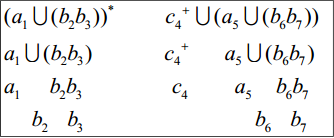
\includegraphics[width=0.5\linewidth]{img/scompo.png}
	\caption{Scomposizione in sottoespressioni}\label{fig:scompo}
\end{figure}